
\begin{figure}[h!]
\centering
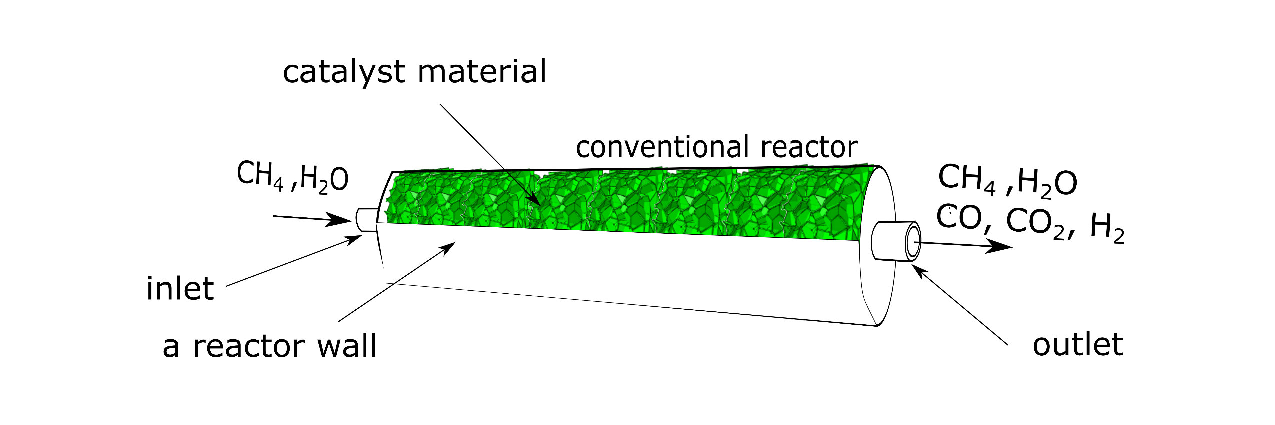
\includegraphics[width=190mm]{conventional-reactor.eps}
\caption{\label{fig:conv_reactor}{Conventional reforming reactor geometry}}
\end{figure}

\begin{figure}[h!]
\centering
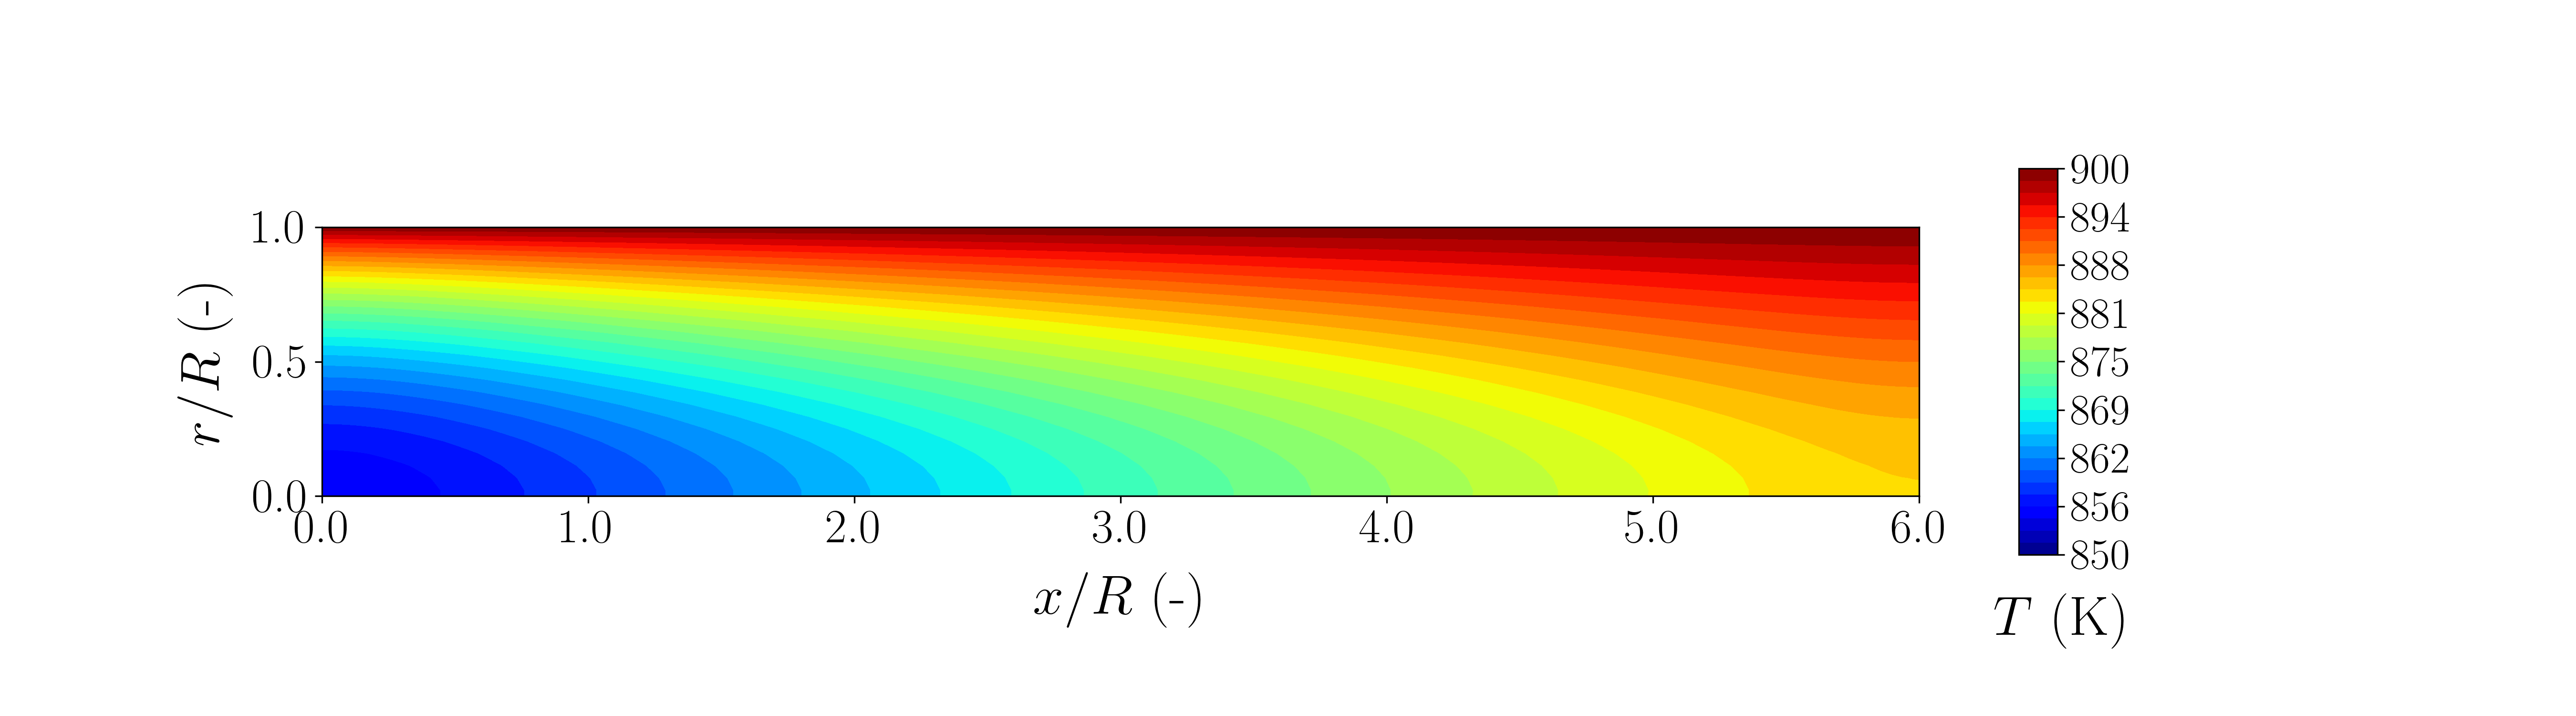
\includegraphics[width=190mm]{ref-Tfield.png}
\caption{\label{fig:conv_reactor_T}{Temperature distribution inside a conventional reforming reactor}}
\end{figure}

The introduction of the macro-pattering concept predicts the division of the catalytic insert in the longitudinal and radial directions. The segments are further filled with either catalytic Ni/YSZ or non-catalytic stainless steel foam. The introduction of the stainless steel foam is expected to allow for a local suppression of the reforming reaction, as the stainless steel is reported to exhibit catalytic at least two orders of magnitude lower when compared to conventional reforming catalysts \cite{Munster1981, Cheekatamarla2006}. Furthermore, the application of metallic foams is used as a measure of altering the temperature distribution. Metallic foams have a significant heat exchange surface contained in a unit volume. Thus, the stainless steel segments are predicted to enhance the temperature distribution not only due to the reduction of the reaction rate but also due to the superior thermal properties. Following, the application of metallic foams requires the implementation of a heat transfer model exclusive to foam structures \cite{Dai2010}. The extraordinary structure of struts and cells has to be taken into account. The model has to allow for a reliable calculation of heat conduction through the material and heat transfer between the metallic foam and the flowing gas.  The most important parameters required for a relevant description regard structural parameters. The morphology of foam structures is investigated via analysis of digital material representations, generated using an in-house procedure, and further quantified using commercial Avizo software \cite{Pajak2021IJHEa}. Conduction of the structural analysis completes the assumptions necessary for the application of the macro-patterning concept. The strategy is addressed in a few different ways. The original approach predicted the division of the reactor into thirty segments of equal length, in the longitudinal direction \cite{Pajak2018}. Further, the reactor is analyzed considering radial division, resulting in five concentric, porous hollow cylinders, with no division in the longitudinal direction. Two different strategies are proposed for the radial division. The first predicts the construction of cylinders with the exact same width of the inlet surface, while the second predicts the exact same inlet surfaces for the cylinder's inlets. Further, the longitudinal segment division is combined with both radial variants, resulting in another two possible strategies. The exact approach and segments definition process is described in Section \ref{sec:react_geom}. A separate numerical analysis is conducted for each of the described ideas. The general idea behind the macro-patterning concept is illustrated in Fig. \ref{fig:react_pattern}. To allow the achievement of uniform temperature distribution, conduction of proper optimization of the segments' alignment is necessary.  The exact subject of the presented study is to define the most relevant approach to the optimization of the segments distribution in the reactor.


\begin{figure}[h!]
\centering
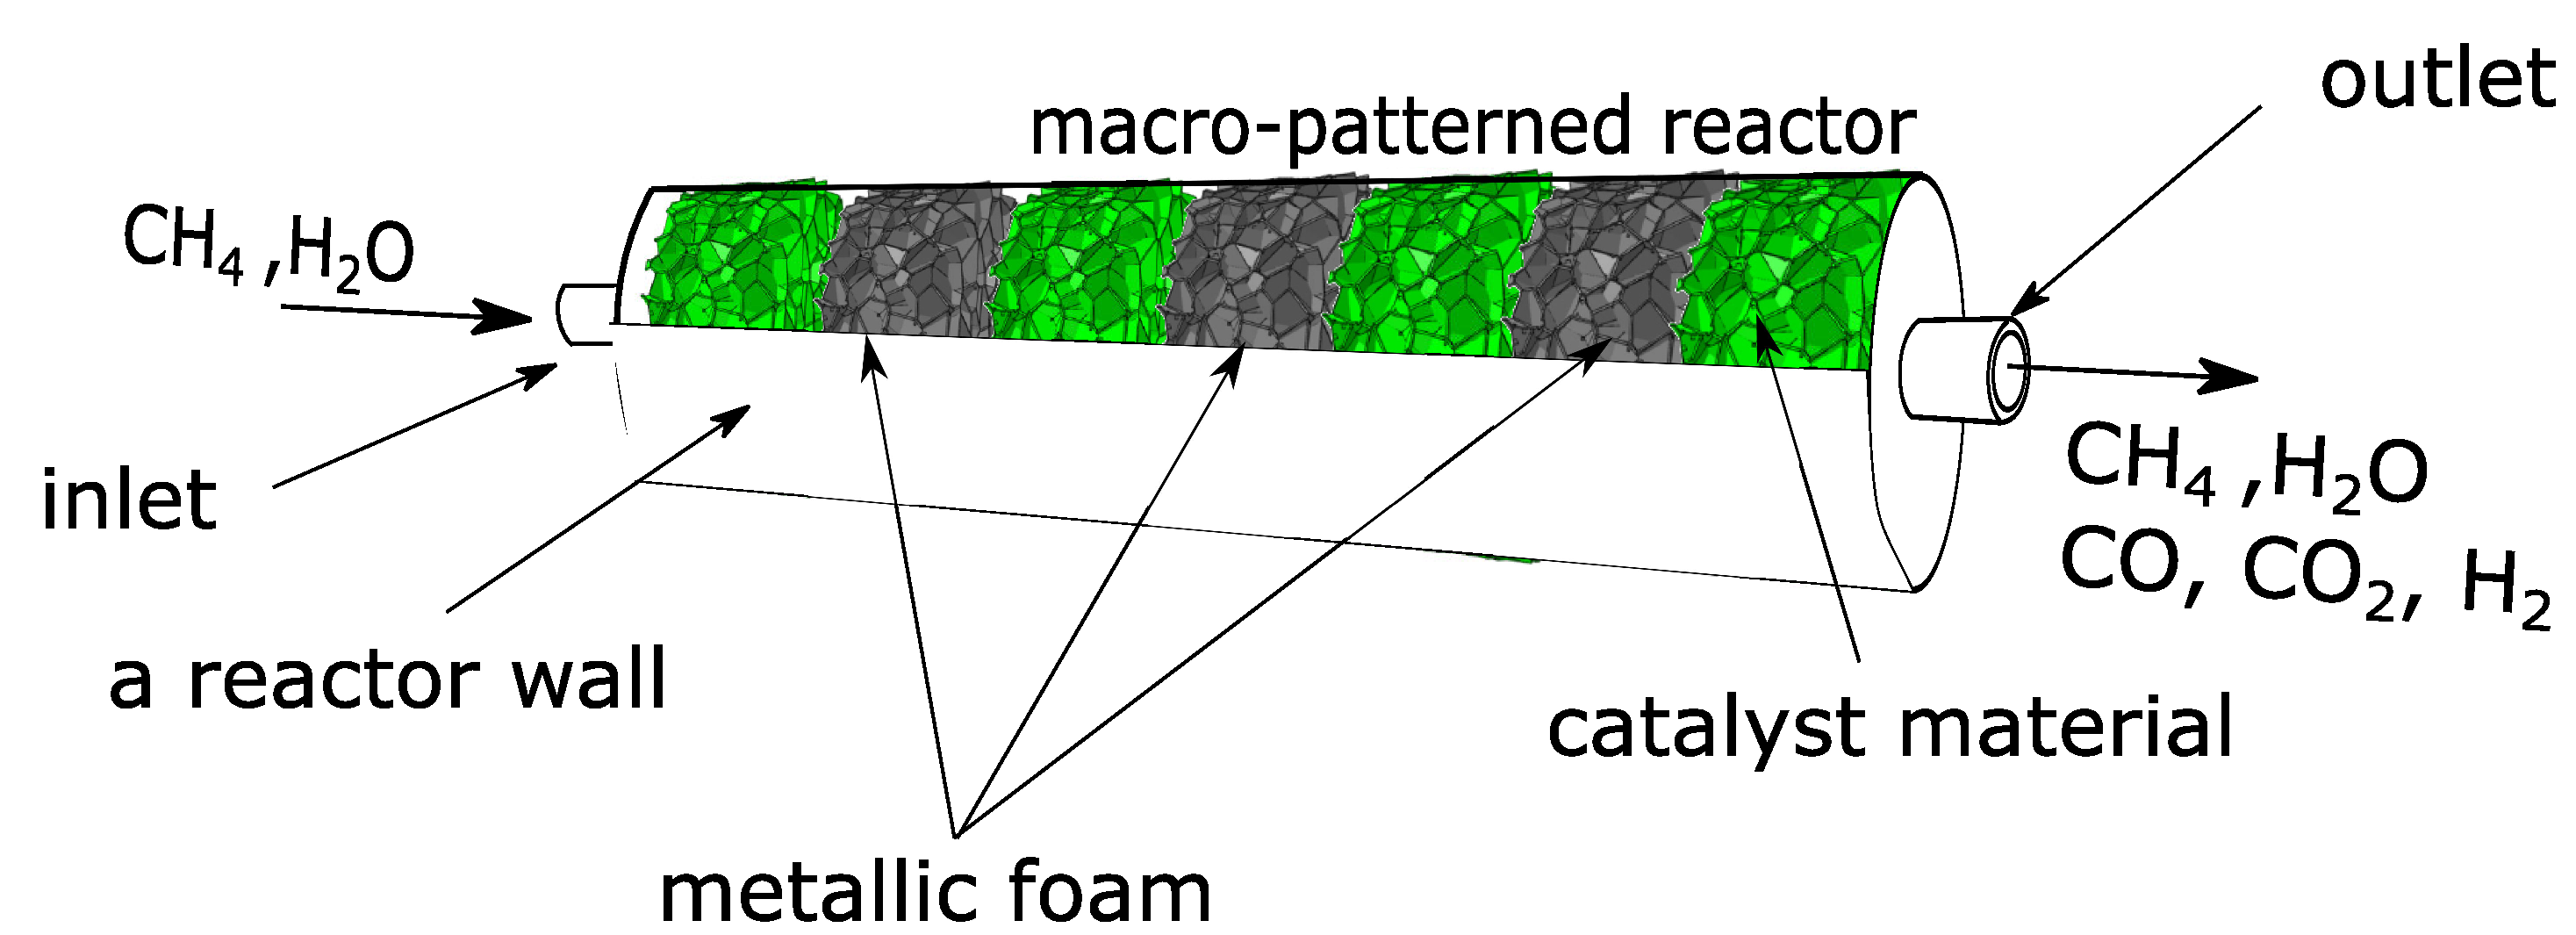
\includegraphics[width=150mm]{macro_geometry.eps}
\caption{\label{fig:react_pattern}{Macro-patterned reactor geometry}}
\end{figure}

\clearpage

Based on the conducted literature review and analysis of the current state of the art, a necessity of optimizing the alignment of the segments is identified. No critical optimization regarding the catalyst distribution in the reforming reactor has been conducted before \cite{Heidebrecht2005, Li2022}. The most advanced investigations are focused on the sensitivity analysis and the adjustment of the process parameters \cite{Rajesh2000, Chen2005, Silva2015}. The optimization procedure is expected to enhance the conditions and effectiveness of an analyzed process or phenomenon. The search for the best solution is conducted through redesigning the conditions, geometry, species composition taking part in the process, etc. The idea of the search for the best solution for a problem has its roots early in the history of mankind. The proofs of the first attempts at the optimization of everyday issues can be found in ancient history.  One of the most recognizable examples is the pursuit of the Greek mathematician Euclid to define the shortest path between two points. Even though the investigation of optimal problems’  solutions started very early, the first proper optimization method was developed by Gauss at the turn of XVIII. Gauss proposed and documented the method of steepest descent used to this day \cite{Curry1944, Meza2010}. Problems regarding optimization can be encountered in each field of science and even in everyday life. The abundance of optimizable phenomena is the reason for the existence of numerous methods and techniques. The procedures may differ in their effectiveness and calculation time \cite{Kusiak2009}. The most conventional approach to the optimization process consists of three steps. The first one predicts the formulation of a proper mathematical model describing be analyzed phenomenon. The second step relies on the definition of fitness functions, which are responsible for the evaluation of the optimization results. The remaining step is the sole optimization procedure itself. The fitness functions are mathematical formulas introduced by the researcher, allowing for deriving a measurable rank for each of the subsequent solutions. The solutions are further evaluated based on the fitness values and the finest is defined as the result of a particular iteration of the optimization procedure \cite{Lange2004}. Basically, the pursuit for the best solution can be brought down to searching for the global minimum or maximum of the fitness function, regarding the considered case. In general, two separate types of the optimization process may be distinguished.  The literature sources define the character of optimization as deterministic or stochastic, depending on the extent of randomness applied to the specific algorithm \cite{Francisco2005}. The deterministic algorithm guarantees convergence in a finite time. However, a certain risk of getting stuck in the local extremum exists. The so-called local extremum trap is a peculiar situation during the analysis of a multi-modal search space. The algorithm falsely recognizes a local extremum as the final step of optimization and terminates the procedure prematurely, as it is unable to break out from the inflection point. Therefore, a deterministic algorithm may be capable of finding a better, but not necessarily the best solution. The reason for the occurrence of the local extremum trap lies down in the principles of the methods. The deterministic algorithms rely on the analysis of the shape of the function’s graph. The stochastic algorithms have a trait for avoiding the local extremum trap, being the introduction of a random factor to the algorithm procedure. Depending on the type of the algorithm, the randomness is introduced to a different extent and in the various parts of specific procedures \cite{Albrecht2003, Spall2012}. The introduction of the random factor serves as a powerful measure for the algorithm to break out from the local extremum, as it enables the procedure to skip freely between parts of the graph if such necessity appears. The selection of a proper optimization procedure character is a vital part of the analysis. To prepare the most robust procedure, a thorough analysis of the optimized problem particularity and conditions has to be conducted. The steam reforming of methane is a widely used technology, but no significant optimization of the process principles has been reported before. The utmost researchers tried to find the best input parameters and alter the operating conditions of the reforming process, like in the research reported by Noureldin et al. or Rajesh et al. \cite{Noureldin2014, Rajesh2000}. However, very few attempts on modifying the reforming unit design and geometry are found. The most advanced research is reported in the article by Heidebrecht and Sundmacher \cite{Heidebrecht2005}. The research regarded optimization of the thermal conditions during a direct internal reforming process inside a molten carbonate fuel cell. The presented model is dimensionless and predicts the division of the fuel cell area into four separate zones, each filled with a catalyst of different densities or activity. Despite the analysis's simplicity, the investigation brought some satisfying results, indicating that the catalyst structure modification is a potentially beneficial solution. Thus, encouraging further investigation of the macro-patterning concept and a deeper analysis of the steam reforming thermal conditions improvement. The subject of the presented thesis's optimization process is to find the best alignment of the catalytic and non-catalytic segments inside the reforming reactor and the segments' morphological parameters. The genetic algorithm is chosen as the optimization technique most suitable for the defined problem \cite{Fouskakis2002}. The genetic algorithm is proven to deal rather effectively with adversely conditioned problems. The algorithm's simplicity and ability to find a global solution are the two main features behind the decision. The genetic algorithm operation is based on evolutionary mechanisms, following the concept of survival of the fittest \cite{Goldberg1989}. In the case of the genetic algorithm, fitness functions are the measure of the evaluation of the specimens and defining the superior ones among the whole population of solutions. The fittest specimens are expected to advance to the next generation and take part in the crossover procedure. The crossover procedure imitates the natural process of gene recombination between the specimens delivering the best results at a certain stage of the optimization process. The algorithm starts its operation by generating an initial population. The specimens being a part of the initial set have the segment parameters entirely randomized. The parameters are further applied to the previously prepared mathematical model used for the calculation of the steam reforming process. Results of   calculation are evaluated by the optimization procedure, assigning a specific fitness for each generated reformer. The amount of processed fuel converted during the reaction and the homogeneity of the temperature field developing inside the reforming reactor are chosen as the most important factors of the analysis. The two features are evaluated based on two separate fitness functions. Regarding the conversion rate, the algorithm aims to maximize the function result, as the level of methane conversion defines the effectiveness of the process. The minimization of the temperature gradients occurring inside the reactor is selected as the second criterion of the analysis. The enhancement of the temperature field distribution inside the reactor is reported to increase the amount of hydrogen contained in the reaction products \cite{Palma2017}. The difference between maximal and minimal temperatures analyzed either locally or globally is chosen as the measure of the magnitude of the gradients.  The previous analyzes indicated that the unification of the temperature field is directly correlated with the difference in the border values of temperature \cite{Pajak2018}. Therefore, the thermal fitness function is minimized by the algorithm. To summarize, the algorithm aims to optimize the design of the macro-patterned reforming reactor catalytic insert. The mutual recombination of the segments’ composition, between specimens among a specific population is expected to deliver results of better quality with each consecutive population. The optimization procedure is continued until optimal values of methane conversion rate and temperature difference are found. Even though a significant part of the algorithm procedure is randomized, the algorithm can not be qualified as a random search method. The genetic algorithms take advantage of the experience gained from preceding calculations to define a new search region, which is expected to contain fitter solutions. Thus, introducing a slight touch of determinism \cite{Goldberg1989}. The presented research regards the optimization of the particular segments distribution and adjustment of morphological parameters, to achieve the highest process efficiency and proper altering of the reforming reaction rate (Chapter \ref{chap:math_model}). Optimization of the given issue is expected to allow the unification of the temperature distribution in the macro-patterned reactor \cite{Pajak2018}. The optimization has to be conducted with respect to maintaining high hydrogen production effectiveness, determining that the problem we are dealing with is a multi-objective optimization. The objectives behave contrarily, as the temperature gradients can only be reduced by limiting the amount of the catalyst used in a particular reactor, which has a consequence in decreasing the methane conversion rate. The less a catalyst is used, the more a reaction rate is diminished. The described problem becomes even more complex if we consider the combinations of possible segment alignments (Chapter \ref{chap:ga}). Some configurations can be falsely recognized as a global optimum when being only an optimal solution in the currently investigated region of the search space. Furthermore, the complexity of the steam reforming simulation results in a considerable computational time, as it combines heat and mass transfer phenomena with the chemical reactions occurring during the process \cite{Brus2012}. Thus, designing a robust optimization procedure is an arduous task. Due to the limited computational capabilities and high cost of the simulation, a fully conventional approach to segment distribution optimization is not possible. The number of specimens in a single generation is exceptionally limited, to allow the computations to deliver results in a finite time. The unconventional approach to the genetic algorithm induces a necessity for a comprehensive investigation of the algorithm conditions and parameters. A complete sensitivity analysis is conducted as the part of the research, to ensure the most suitable optimization strategy, considering the steam reforming reaction.









%%%%%%%%%%%%%%%%%%%% MATH MODEL %%%%%%%%%%%%%%%%%%%%%%%%%%%%%%%%%%%%%%%

The method of volume averaging is applied to compose the governing equations, as a flow through porous media is considered \cite{Whitaker1999, Brus2014}.


